\documentclass[12pt,a4paper]{article}
\usepackage[a4paper, total={6in, 9in}]{geometry}
\usepackage{tikz}
\usetikzlibrary{shapes,backgrounds}
\usepackage[utf8]{inputenc}

\title{Exercise 1} 
\author{KLMED8004: Medical Statistics, Part 1\\\\ John Zobolas (Ioannis Zompolas)\\ PhD Candidate, Department of Biology}
\date{September 2018}

\begin{document}

\maketitle

\section*{Task 1 \& Task 2}
See: \textbf{exe01\_Tasks1and2\_JohnZobolas.Rmd}
(or the .html file of the produced report)

\section*{Task 3}

\subsection*{Problems 3.136-3.140}
The sample size in this cardiovascular disease study is $N=446$. Below is \textbf{Table 3.22} where the association between the blood-pressure index (AAI) and the S-T segment depression of the electrocardiogram (ECG) is shown:

\begin{center}
\begin{tabular}{ c c c }
 & & S-T segment depression \\ \hline
 & + & - \\ \hline  
 $AAI < 1.0$ & 20 & 95 \\
 $AAI \geq 1.0$ & 13 & 318 
\end{tabular}
\end{center}

Since $AAI < 1.0$ signifies a test-positive for heart disease while the golden standard for the same disease is the positive $(+)$ S-T segment depression, we have that: $TP=20, FN=13, FP=95, TN =318$.
So, the positives and negatives are: $P=TP+FN=33, N=TN+FP=413$. 
Thus we can calculate:
$$Sensitivity=\frac{TP}{P}=\frac{20}{33}=0.6$$

$$Specificity=\frac{TN}{N}=\frac{318}{413}=0.77$$
Since the subjects in the study are a random sample from Japan's population, we can calculate the disease prevalence as:
$$x=P(Positives)=\frac{P}{N}=\frac{33}{446}=0.074$$

So, the predictive value positive and predictive value negative can be calculated as:

$$PV^+=\frac{Sensitivity\cdot x}{Sensitivity\cdot x + (1-Specificity)\cdot (1-x)}=$$
$$=\frac{0.6\cdot 0.074}{0.6\cdot 0.074 + (1-0.77)(1-0.074)}=0.17$$

$$PV^-=\frac{Specificity\cdot (1-x)}{Specificity\cdot (1-x) + (1-Sensitivity)\cdot x}=$$
$$=\frac{0.77\cdot (1-0.074)}{0.77\cdot (1-0.074) + (1-0.6)\cdot0.074}=0.96$$
\\
These results show that the AAI test is not a good indicator of heart disease since the $PV^+$ is very small, meaning that we are only $17\%$ sure that a person has heart disease given that his test resulted in: $AAI\leq1.0$. Even with better technology for testing the AAI index and given that the sensitivity thus increased to let's say $0.8$, we would still have a low positive predictive value: $PV^+(Sensitivity=0.8)=22\%$.

\subsection*{Problems 3.12-3.15}
We are considering a family with two parents and two children. Let the events of interest be: $A_1$=\{mother has the influenza\}, $A_2$=\{father has the influenza\}, $A_3$=\{the first child has the influenza\} and $A_4$=\{the second child has the influenza\}. It is given that: $P(A_1)=P(A_2)=0.1, P(A_1\cap A_2)=0.02$ and that: $P(A_3)=P(A_4)=0.2, P(A_3\cap A_4)=0.1$.

\begin{description}
  \item[$\bullet$] Are the events $A_1,A_2$ independent? No, since:
  $$P(A_1)\cdot P(A_2)=0.01\neq P(A_1\cap A_2)=0.02$$
  \item[$\bullet$] What is the probability that at least one child will get the influenza?
  $$P(A_3\cup A_4)=P(A_3)+P(A_4)-P(A_3\cap A_4)=0.2+0.2-0.1\\=0.3=30\%$$
  \item[$\bullet$] What is the conditional probability that the father has the influenza given that the mother has influenza?
  $$P(A_2|A_1)=\frac{P(A_1\cap A_2)}{P(A_1)}=\frac{0.02}{0.1}=20\%$$
  \item[$\bullet$] What is the conditional probability that the father has the influenza given that the mother does not have influenza?
  $$P(A_2|\overline{A_1})=\frac{P(\overline{A_1}\cap A_2)}{P(\overline{A_1})}=\frac{P(A_2)-P(A_1\cap A_2)}{1-P(A_1)}=\frac{0.1-0.02}{1-0.1}=8.8\%$$
  Note: The above results make perfect sense since they show that it is more probable for the father to have influenza given that his wife also has.
\end{description}

\section*{Task 4}

\subsection*{Problems 3.76-3.78}
In this hypertension study, the measurement is the change in blood pressure before and after a stimulating experience. There is strong cardiovascular reactivity if: $\Delta DBP\geq 10$ mm Hg. In the next \textbf{Table 3.11}, we can see the classification of the cardiovascular reactivity using an automated as well as a manual sphygmomanometer:
\begin{center}
\begin{tabular}{ c c c }
 & & $\Delta DBP$, manual \\ \hline
 $\Delta DBP$, automated & $< 10$ & $\geq 10$ \\ \hline  
 $< 10$ & 51 & 7 \\
 $\geq 10$ & 15 & 6 
\end{tabular}
\end{center}

It's easy to see that the sample size is $N=51+7+15+6=79$. Now, since the automated measurements signify the test-positives for cardiovascular reactivity whereas the manual measurements are considered the "true" measurements, we have that: $TP=6, FN=7, FP=15, TN =51$. So, the positives and negatives are: $P=TP+FN=13, N=TN+FP=66$. Thus we can calculate:
$$Sensitivity=\frac{TP}{P}=\frac{6}{13}=0.46$$

$$Specificity=\frac{TN}{N}=\frac{51}{66}=0.77$$
Since the population tested is representative of the general population, we can calculate the disease prevalence as:
$$x=P(Positives)=\frac{P}{N}=\frac{13}{79}=0.164$$

So, the predictive value positive and predictive value negative can be calculated as:

$$PV^+=\frac{Sensitivity\cdot x}{Sensitivity\cdot x + (1-Specificity)\cdot (1-x)}=$$
$$=\frac{0.46\cdot 0.164}{0.46\cdot 0.164 + (1-0.77)(1-0.164)}=0.28$$

$$PV^-=\frac{Specificity\cdot (1-x)}{Specificity\cdot (1-x) + (1-Sensitivity)\cdot x}=$$
$$=\frac{0.77\cdot (1-0.164)}{0.77\cdot (1-0.164) + (1-0.46)\cdot0.164}=0.88$$

\section*{Task 5}

\subsection*{Problems 4.5-4.6}

Selecting $k=5$ out of $n=50$ cases of angina, when order matters, is:
$$N=50\cdot49\cdot48\cdot47\cdot46$$
If the order of selection does not matter, then:
$$N^{'}={n \choose k}={50 \choose 5}=\frac{50!}{5!\cdot45!}$$

\section*{Task 6}

\subsection*{Problems 4.1-4.3}

$X$ is a random variable representing then number of hypertensive adults (HT) in a family (mother and father). We consider someone as having HT, if their blood pressure is: $DBP\geq90$. It is given that the events $A$=\{mother is HT\} and $B$=\{father is HT\} are \textbf{independent} and the probabilities are: $P(A)=0.1,P(B)=0.2$. So, we can calculate the probability of \textit{both of them} being HT as: $P(A\cap B)=P(A)\cdot P(B)=0.1\cdot 0.2=0.02$ and the probability of \textit{at least one of them} being HT as: $P(A\cup B)=P(A)+P(B)-P(A\cap B)=0.28$.

We will now derive the probability mass function (pmf) of the random variable $X$. The possible values are 0, 1 and 2 representing that none is HT in the family, only one is or that both of the adults are. Using the next Venn diagram it's easy to calculate the probabilities needed: 
\begin{center}
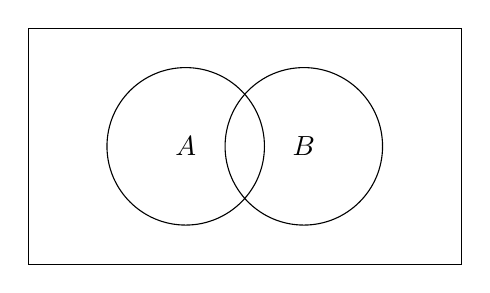
\begin{tikzpicture}
\draw (-2,-1.5) rectangle (3.5,1.5);
\draw (0,0) circle (1cm) node {$A$};
\draw (1.5,0) circle (1cm) node {$B$};
\end{tikzpicture}
\end{center}

\begin{description}
  \item[$\bullet$] $P(X=0)=1-P(A\cup B)=1-0.28=0.72$
  \item[$\bullet$] $P(X=1)=P(A\cup B)-P(A\cap B)=0.28-0.02=0.26$
  \item[$\bullet$] $P(X=2)=P(A\cap B)=0.02$
\end{description}

So, the pmf can be described with the next table:

\begin{center}
\begin{tabular}{ c | c | c | c}
 $k$ & 0 & 1 & 2 \\ \hline
 $P(X=k)$ & 0.72 & 0.26 & 0.02
\end{tabular}
\end{center}

Next, we can calculate the expected value and variance:
$$\mu=E(X)=\sum_{k=0}^2 k P(X=k)=0.3$$
$$\sigma^2=Var(X)=\sum_{k=0}^2 k^2 P(X=k) - \mu^2=0.25$$

\section*{Task 7}

\subsection*{Problems 4.9-4.10}
In this problem, we have $k=6$ out of $n=15$ students in a grade-school class that developed influenza ($40\%$ of them were affected by the disease). The probability that you will get influenza nationwide is $p=0.2=20\%$. Does this means that there is an excessive number of infected students in that class? \\\\
Let $X$ be a random variable representing the number of students that have influenza (in that class). We will use the \textbf{binomial distribution} where each independent trial asks a student if he/she has the influenza with probability $p=0.2$. Our initial hypothesis here is that this class is representative of the natiowide population and as such, these excessive cases of influenzas are not worrying. We will calculate the probability of having at least 6 students with influenza: 
$$P(X\geq 6)=\sum_{k=6}^{15} {15 \choose k}0.2^k\cdot (1-0.2)^{15-k}$$

We will use the $R$ function: $pbinom(k, size, prob) = P(X\leq k|size=n, prob=p)$ for ease of calculation. So: $P(X\geq 6)=1-P(X\leq 5)=1-pbinom(5, size=15, prob=0.2)\approx 0.061=6\%$, which is larger than the standard significance level of $5\%$, indicating thus that the results are not statistically significant and  \textbf{there is no need to worry} about the excessive number of infected students (we accept the initial hypothesis). 

The expected number of infected students is given by the expected value of the binomial distribution: $\mu=E(X)=n\cdot p=15\cdot 0.2=3$ students.

\section*{Task 8}

\subsection*{Problems 4.89-4.91}

Let $X$ be a random variable that represents the number of admissions to the Emergency Room (which follows the \textbf{Poisson distribution}). The rate of admissions is on average $\lambda_1=2$ admissions/day if it is a weekday and $\lambda_2=1$ admission/day if it is a weekend day (Saturday or Sunday). We will use the next two $R$ functions for ease of calculation: 
$$dpois(k, \lambda) = P(X=k)=\frac{\lambda^k\cdot e^{-\lambda}}{k!}$$
$$ppois(k, \lambda) = P(X\leq k)=\sum_{n=0}^{k} \frac{\lambda^n\cdot e^{-\lambda}}{n!}$$

\begin{description}
  \item[$\bullet$] What is the probability of at least one admission on a Wednesday?
  $$P(X\geq 1|Wednesday)=1-P(X=0|Wednesday)=$$
  $$=1-dpois(0, lambda=2)=0.86=86\%$$
  \item[$\bullet$] What is the probability of at least one admission on a Saturday?
  $$P(X\geq 1|Saturday)=1-P(X=0|Saturday)=$$
  $$=1-dpois(0, lambda=1)=0.63=63\%$$
  So, the probability of getting at least one admission is greater on a weekday which makes sense, since the average rate of admissions/day is twice as much compared to a weekend day.
  \item[$\bullet$] What is the probability of having 0, 1 and 2+ admissions for an entire week, if the results for different days during the week are assumed to be independent?
  \\\\
  Since we have $\lambda_1=2$ admissions/day if it is a weekday and $\lambda_2=1$ admission/day if it is a weekend day, we expect that we will have $\lambda_1*5+\lambda_2*2=12$ admissions/week, since the results are independent for each day. So:
  \\\\
  $P(X=0|$all week$)=P(X=0|\lambda=12)=6.144212 \cdot 10^{-6}$
  \\\\
  $P(X=1|$all week$)=P(X=1|\lambda=12)=7.373055 \cdot 10^{-5}$
  \\\\
  $P(X\geq2|$all week$)=1-[P(X=0|$all week$)+P(X=1|$all week$)]=0.9999201\simeq 99.99\%$
\end{description}
\end{document}